\documentclass[twocolumn,a4paper]{article}
\usepackage[margin=1in,footskip=0.25in]{geometry}
\providecommand{\keywords}[1]{\textbf{{Keywords: }}#1}
 \usepackage{bibentry} %% to have the publications listed where they are supposed 
\usepackage{comment}
\usepackage[utf8]{inputenc}
\usepackage{graphicx}
\usepackage[numbers]{natbib}
\usepackage{url}

\usepackage{authblk}
\newcommand*{\affaddr}[1]{#1} % No op here. Customize it for different styles.
\newcommand*{\affmark}[1][*]{\textsuperscript{#1}}
\newcommand*{\email}[1]{\texttt{#1}}
\usepackage{graphicx}
\graphicspath{ {images/} }

\usepackage{sectsty}
\allsectionsfont{\centering}


\begin{document}


\title{Automatic Extraction of TEI Structures in Digitized Lexical Resources using Conditional Random Fields}  
\author{%
Mohamed Khemakhem\affmark[1,2,3], {Luca Foppiano\affmark[1] and Laurent Romary\affmark[1,2]\\
\affaddr{\affmark[1]Inria - Alpage, Paris}\\
\affaddr{\affmark[2]Centre Marc Bloch, Berlin}\\
\affaddr{\affmark[3]Université Paris Diderot, Paris}\\
\email{\{mohamed.khemakhem,luca.foppiano,laurent.romary}\}@inria.fr}\\
}
%\maketitle

%\section{Introduction}

\paragraph{}An important number of digitized lexical resources remain unexploited due to their unstructured content. Structuring manually such resources is a costly task due to their multifold complexity. Our goal is to find an approach for automatically structuring digitized dictionaries, independently from the language or the lexicographic school or style. We present \textbf{GROBID-Dictionaries}%\footnote{Available at \url{https://github.com/MedKhem/grobid-dictionaries} under the Apache License.}, an open source machine learning system for structuring lexical resources. 	
%\section{Approach}
 
\paragraph{} Our approach is twofold: we perform a cascading structure extraction, while we select in each level specific features for training.

 We followed a "divide to conquer" strategy to dismantle the structure of a digitized dictionary, based on the observation of its text layout. Main pages (see Figure 1) in almost any  dictionary share three blocks: a header (green), a footer (blue) and a main body (orange). In a second level, a set of lexical entries (red) forms the body. In a third stage (see Figure 2), an entry could contain zero or many: form (green), etymology (blue), sense (red) or/and related entry. The same logic could be applied further for each extracted block but in the scope of this paper we focus just on the first three levels.  
 \begin{figure}
\framebox{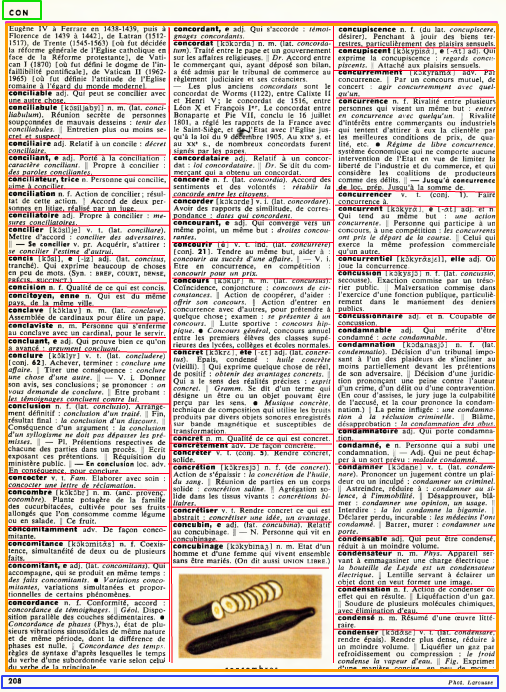
\includegraphics[width=\columnwidth]{larousse-colored.png}} 
%\caption{First and second levels\label{fig:mouseover}}
\end{figure}
\begin{figure}
\framebox{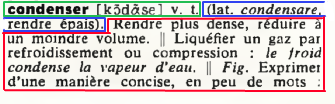
\includegraphics[width=\columnwidth]{larousse-entry-colored.png}} 
%\caption{Third level\label{fig:mouseover}}
\end{figure}  
 
 Such cascading approach ensures a better understanding of the learner's output and consequently simplifies the vital feature selection process. Limited exclusive text blocks per level helps significantly in diagnosing the cause of prediction errors. It allows an early detection and replacement of irrelevant selected features that can bias a trained model. 
 
 In such a segmentation, it becomes more straightforward to notice that, for instance, the token position in the page is very relevant to detect headers and footers and has almost no pertinence for capturing a sense in a lexical entry which is very often split on two pages.  




%\section{Grobid \& CRF} 
\paragraph{}To implement our approach, we were based on GROBID~\cite{Lopez2015GROBIDI}, a machine learning system adopting the same logic but for the extraction of bibliographical metadata.  GROBID relies on Conditional Random Fields (\textbf{CRF})~\cite{lavergne2010practical} to label text sequences. Another asset to use GROBID is that the used labels are XML elements from \textbf{TEI}, a de-facto standard that dedicates a whole chapter for encoding dictionaries~\cite{budin2012creating}. Consequently, the need to reformat the resulting segmentation is bypassed.
%\section{Experiment and Results}
 
\paragraph{}Our experiments justify so far our choices, where models for the first two levels trained on two different dictionary samples have given a high precision and recall with a small amount of annotated data. Relying mainly on the text layout, we tried to diversify the selected features for each model, on the token and line level. We are working on tunning features and annotating more data to maintain the good results with new samples and to improve the third segmentation level.  

%\section{Related works}
 
\paragraph{}While just few task specific attempts~\cite{bago2015using}. have been using machine learning in this research direction, the landscape remains dominated by rule based techniquess~\cite{khemakhem2009towards,fahmy2014towards,mykowiecka2012building} which are ad-hoc and costly, even impossible, to adapt for new lexical resources.
	


\bibliographystyle{plainnat}
%\bibliography{Full_Desc}

\end{document}
